\chapter{Resultados e Discuss�es}
\label{Resultados}

\par Os s�mbolos a serem classificados s�o mostrados na figura~\ref{fig:simbolos}.

\begin{figure}
	\centering
	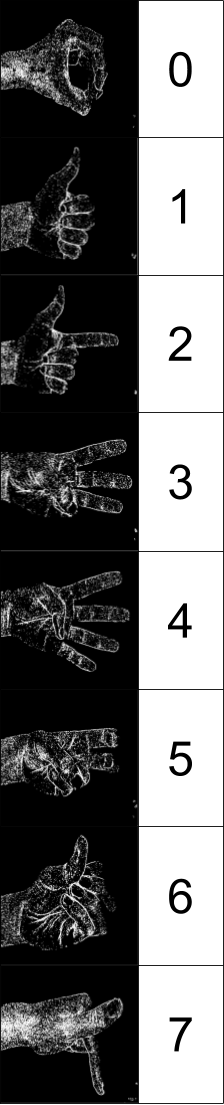
\includegraphics[height=\textheight]{./Resources/Maos_numeros.png}
	\caption{S�mbolos propostos para o sistema de classifica��o.}
	\label{fig:simbolos}
\end{figure}

\par O sistema funciona com baixas taxas de erro quando trabalha com poucos s�mbolos, no entanto o processo de classifica��o se torna impreciso conforme a quantidade de s�mbolos diferentes aumenta. A figura~\ref{fig:erro} mostra a taxa de erro obtida em fun��o da quantidade de s�mbolos diferentes que foram adicionados ao banco de dados.

\begin{figure}[H]
	\centering
	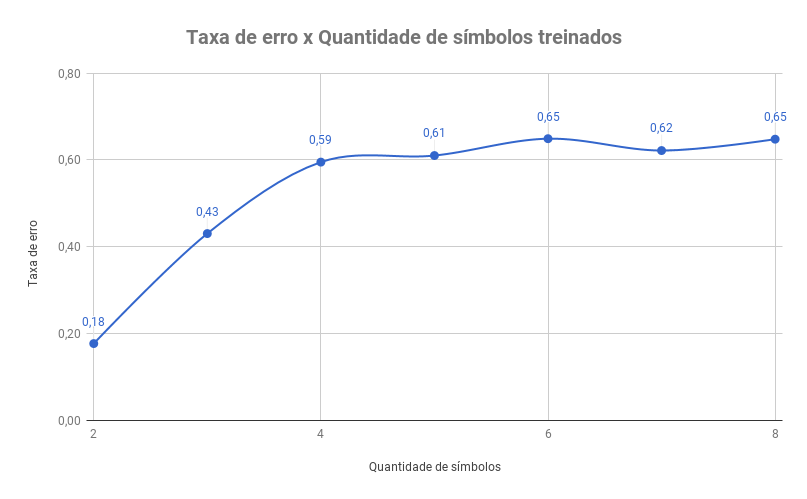
\includegraphics[width=\textwidth]{./Resources/grafico_erro.png}
	\caption{Diagrama simplificado do sistema.}
	\label{fig:erro}
\end{figure}

\par Para realizar os testes, o banco de dados foi treinado com a mesma quantidade de exemplos para cada s�mbolo (3 exemplos) e foi dada como entrada a mesma quantidade de inst�ncias de cada s�mbolo (3 inst�ncias para cada s�mbolo treinado). O gr�fico representa a taxa de desequil�brio entre o esperado e o obtido.

\par Como mostardo na figura~\ref{fig:erro}, acima de 2 s�mbolos o sistema � ca�tico, com baixas taxas de acerto. Esse resultado indica duas possibilidades para que o sistema n�o funcione como o esperado:
\begin{enumerate}
	\item O processo de \textit{hash} elimina muitas caracter�sticas da imagem de forma que diferenciar muitas imagens se torna uma tarefa complicada.
	\item O classificador utilizado (\textit{K-NN}) n�o � bom o suficiente para classificar muitos s�mbolos.
\end{enumerate}

\par Muito embora o classificador \textit{K-NN} seja bastante simples se comparado �s t�cnicas utilizadas nos trabalhos citados anteriormente, a transforma��o \textit{hash} � a principal respons�vel pelos resultados obtidos, uma vez que caracter�sticas importantes da imagem s�o descartadas neste processo.
\par Isso ficou evidente em um segundo teste realizado com um novo conjunto de s�mbolos.


